\documentclass[a4paper,12pt]{article}

% Packages
\usepackage{geometry}
\usepackage{graphicx}
\usepackage{amsmath}
\usepackage{caption}
\usepackage{subcaption}
\usepackage{listings}
\usepackage{float}
\usepackage{hyperref}
\usepackage{circuitikz}

% Page setup
\geometry{margin=1in}

\begin{document}

\begin{figure}[H]
   \centering
   
\includegraphics[width=0.8\textwidth]{./images.png}
\end{figure}

\begin{center}
    Year : 2023-24 \\
    Subject Code : EE1200 \\
    Branch : Electrical Engineering \\
    Name : Aditi Dure 
\end{center}

\newpage
\title{Low pass and High pass filter}
\date{}
\maketitle

\section{Aim}
To plot Frequency response of low pass and high pass filters

\section{Apparatus}
\subsection{Equipments}
\begin{enumerate}
\item Function Generator
\item Bread Board
\item Oscilloscope
\item Multimeter
\end{enumerate}
\subsection{Components}
\begin{enumerate}
\item Resistor($150\, \text{k}\Omega$)
\item Capacitor($220\, \text{pF}$)
\end{enumerate}

\section{Circuit Diagram}
\subsection{Low pass}
\begin{center}
\begin{circuitikz}
    \draw (0,0)
    to[sV, v=$V_{\text{in}}$] (0,2)
    to[R, l=$\ 150k \Omega$] (2,2)
    to[C, l=$220pF$] (2,0)
    -- (0,0);
    
    \draw (2,2) -- (4,2) node[ocirc] (Vout) {} node[anchor=south west, midway] {$V_{\text{out}}$};
    \draw (2,0) -- (4,0) node[ground] {};
\end{circuitikz}
\end{center}

\subsection{High Pass}
\begin{center}
\begin{circuitikz}
    \draw (0,0)
    to[sV, v=$V_{\text{in}}$] (0,2)
    to[C, l=$220pF$] (2,2)
    to[R, l=$\ 150k \Omega$] (2,0)
    -- (0,0);
    
    \draw (2,2) -- (4,2) node[ocirc] (Vout) {} node[anchor=south west, midway] {$V_{\text{out}}$};
    \draw (2,0) -- (4,0) node[ground] {};
\end{circuitikz}
\end{center}

\section{Theory}
\begin{enumerate}
\item An RC low-pass filter allows signals with frequencies below a certain cutoff frequency to pass through while attenuating higher frequencies.
\item As the frequency of the input signal approaches the cutoff frequency, the output amplitude of the low-pass filter gradually decreases.
\item Conversely, an RC high-pass filter allows signals with frequencies above a certain cutoff frequency to pass through while attenuating lower frequencies.
\item As the frequency of the input signal increases beyond the cutoff frequency, the output amplitude of the high-pass filter gradually increases.
\end{enumerate}

\section{Procedure}
\begin{enumerate}
\item Set up the circuit as shown taking the output across the capacitor (resistor for high pass filter).
\item The input for the filter is taken from output of function generator. It is connected to channel 2 of oscillator.
\item Vary the frequency of the input signal over a wide frequency range (keeping the input amplitude fixed). Note the value of each frequency.
\item Plot the values of gain vs Frequency and find out cut-off frequency from it. (higher cutoff for low pass filter and lower cutoff for high pass filter.)
\end{enumerate}

\section{Calculations}
\begin{enumerate}
\item Firstly, let us find the cutoff frequency theoretically:
\begin{align}
f &= \frac{1}{2\pi RC} \\
&= \frac{1}{2\pi\cdot 150\cdot 10^3 \cdot 220\cdot 10^{-12}} \\
&= 4825.32 \text{Hz}
\end{align}
\item Now find corresponding $V_\text{out}$ for corresponding frequencies and note it down in a table as shown below. \\
Let $V_\text{in}$ be 5V.

%values to be added yet

\begin{table}[H]
  \centering
  \begin{tabular}{|c|c|c|c|}
    \hline
    \textbf{Frequency} & \textbf{$V_\text{out}$(in V)} & \textbf{$A(gain)=\frac{V_\text{out}}{V_\text{in}}$} & \textbf{Frequency response=$20logA$(in dB)} \\
    \hline
    500Hz & 4.984 & 0.997 & -0.17\\
    \hline
    1KHz & 4.970 & 0.994 & -0.34\\
    \hline 
    2KHz & 4.942 & 0.988 & -0.68\\
    \hline
    4KHz & 4.887 & 0.976 & -1.36\\
    \hline
    5KHz & 4.849 & 0.970 & -1.70\\
    \hline
    6KHz & 4.810 & 0.963 & -2.03\\
    \hline
    10KHz & 4.704 & 0.941 & -3.40\\
    \hline
  \end{tabular}
  \caption{Observation Table for Low Pass}
\end{table}

\begin{table}[H]
  \centering
  \begin{tabular}{|c|c|c|c|}
    \hline
    \textbf{Frequency} & \textbf{$V_\text{out}$(in V)} & \textbf{$A(gain)=\frac{V_\text{out}}{V_\text{in}}$} & \textbf{Frequency response=20logA(in dB)} \\
    \hline
    500Hz & 1.86 & 0.372 & -19.81 \\
    \hline
    1KHz & 2.53 & 0.506 & -13.64\\
    \hline 
    2KHz & 3.30 & 0.66 & -8.33\\
    \hline
    4KHz & 4.10 & 0.82 & -3.96\\
    \hline
    5KHz & 4.37 & 0.874 & -2.68\\
    \hline
    6KHz & 4.51 & 0.902 & -2.05\\
    \hline
    10KHz & 4.80 & 0.96 & -0.79\\
    \hline
  \end{tabular}
  \caption{Observation Table for High Pass}
\end{table}

\item Now plot a graph of frequency response versus frequency

\begin{figure}[H]
    \centering
    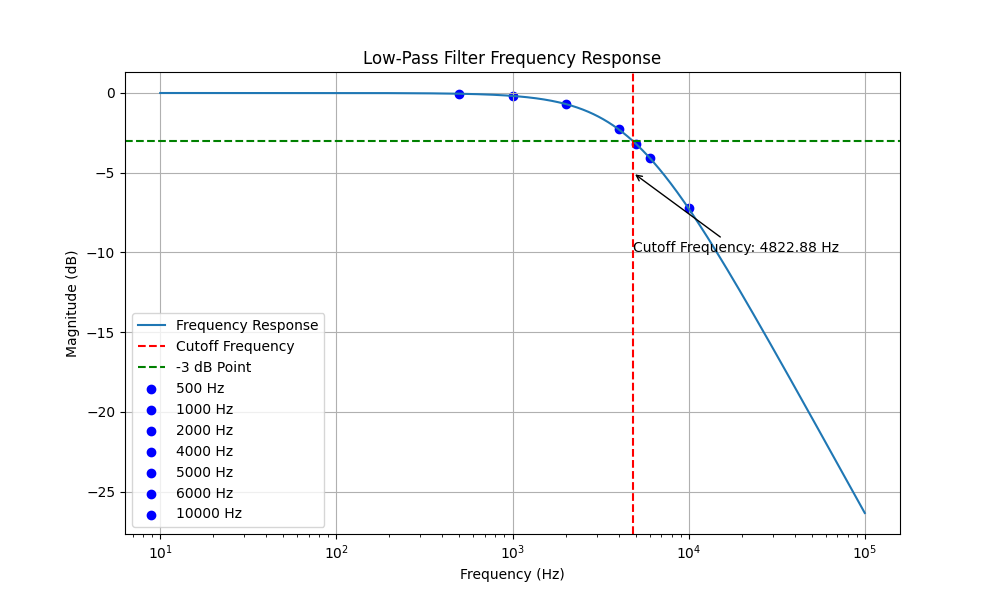
\includegraphics[width=0.8\textwidth]{1.png}
    \caption{For Low pass filter}
    \label{fig}
\end{figure}

\begin{figure}[H]
    \centering
    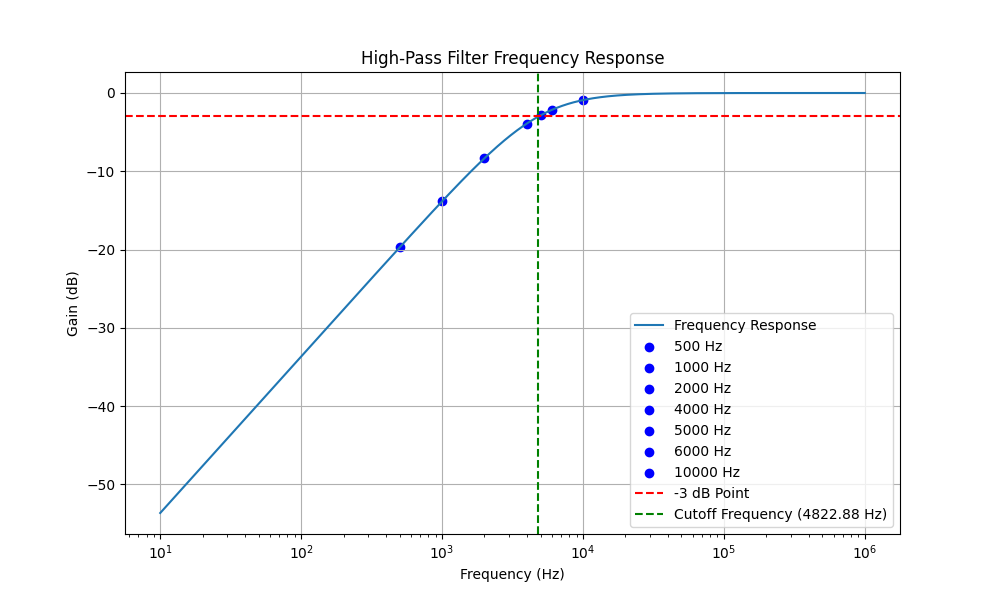
\includegraphics[width=0.8\textwidth]{2.png}
    \caption{For High pass filter}
    \label{fig}
\end{figure}

\item Cutoff frequency now corresponds to frequency response being -3dB i.e. 4822.88Hz. 
\end{enumerate}

\section{Result}

\begin{table}[H]
  \centering
  \begin{tabular}{|c|c|}
    \hline
    caculated & measured \\
    \hline
    4825.32Hz & 4822.88Hz  \\
    \hline
  \end{tabular}
  \caption{Result}
\end{table}

\end{document}

